%Style Section
\documentclass{article}
\usepackage{latexsym, amsmath, amssymb, enumitem}
\usepackage{hyperref}
\usepackage{tikz}
\usepackage{bussproofs}
\usepackage{graphicx}
\graphicspath{ {/} }
%\usepackage[dvips]{graphicx}
\usepackage[left=2.5cm,right=2.5cm,top=2.5cm,bottom=2.5cm]{geometry}

%Declaration Section
\newtheorem{Corollary}{Corollary}
\newtheorem{Proposition}{Proposition}
\newtheorem{Lemma}{Lemma}
\newtheorem{Definition}{Definition}
\newtheorem{Theorem}{Theorem}
\newtheorem{Example}{Example}

%Command Section
%\errorcontextlines=0
%\numberwithin{equation}{equation}

\newcommand{\R}{{\mathbb R}}
\newcommand{\C}{{\mathbb C}}
\newcommand{\N}{{\mathbb N}}
\newcommand{\Q}{{\mathbb Q}}
\newcommand{\Z}{{\mathbb Z}}
\newcommand{\re}{\textrm{re}}
\newcommand{\im}{\textrm{im}}
\newcommand{\Stab}{\textrm{Stab}}
\newcommand{\Var}{\textrm{Var}}
\newcommand{\Int}{\textrm{Int}}
\newcommand{\Bd}{\textrm{Bd}}
\newcommand{\br}{\mathbf r}
\newcommand{\g}{\mathbf g}
\newcommand{\h}{\mathbf h}
\newcommand{\w}{\mathbf w}
\newcommand{\X}{\mathbf X}
\newcommand{\x}{\mathbf x}
\newcommand{\z}{\mathbf z}
\newcommand{\bbeta}{\boldsymbol{\beta}}

%Special for Tests
\newcounter{Task}
\setcounter{Task}{1}
\newenvironment{Task}
{\medskip \noindent{\bf Task \theTask.}\addtocounter{Task}{1}}
%{\smallskip}

\title{Estimating the effect of US Food Aid on Civil Conflict}
\author{Lawrence Chan}
\date{December 11th, 2017}

\begin{document}
\maketitle
\begin{abstract}
We duplicate the results of Nunn and Qian (2014), who use lagged wheat production as an instrument for US food aid to conclude that US food aid increases the chance of civil (intrastate) conflict.  Interestingly, with a slightly different way of performing the controls, we find a significant negative effect of food aid on international conflict, in addition to similar results on civil conflict. In addition, we test for heteroscedasticity, and find that their assumption of homoscedasticity for reporting $p$-values is invalid. Finally, we test for endogeneity, and find evidence of endogenous variables in their OLS regression.
\end{abstract}
\section{Introduction}
There has been much debate about the effects of food aid from developed countries toward the developing world. Nunn and Qian's 2014 Paper, “US Food Aid and Civil Conflict”, uses a 2SLS regression (using shocks in the US agricultural market as an instrument to aid) and several robustness checks to conclude that US food aid increases the incidence and duration of civil conflicts.\\

In this work, we duplicate their analysis (with minor differences in control variables) and then perform additional tests for heteroscedasiticity and endogeneity. \footnote{Our code and data are available online at \href{https://github.com/chanlaw/USFoodAidConflict}{https://github.com/chanlaw/USFoodAidConflict}. In addition, our code is attached as an appendix. } We find some evidence of heteroscedasiticty and for US wheat aid being endogenous. One of their main results  - that US Wheat Aid significiantly increases the incidence of all wars in a country - disappears after switching to heteroscedasiticty-robust standard errors. This suggests that their results may not be particularly robust.

\section{Description of Dataset and Preliminary Analysis}
Before jumping in to the discussion of Nunn and Qian's main results, we describe the datasets being used and provide some preliminary analysis.\\

The two main datasets are the UCDP/PRIO Armed Conflict Dataset and Food and Agriculture Organization’s (FAO) FAOSTAT database. The dependent variables include the prevalence of war, defined as any armed conflict leading to more than 25 deaths, as well as civil and interstate war. The authors use US wheat aid as a proxy for US food aid, and wheat production from the previous year as an instrument for . We used the merged data set provided by the authors\footnote{Available at the AER website here: \href{https://www.aeaweb.org/articles?id=10.1257/aer.104.6.1630}{https://www.aeaweb.org/articles?id=10.1257/aer.104.6.1630}}, which contains 4089 observations across 125 OECD countries over the period of 36 years from 1971 to 2006. (The actual dataset contains quite a few more rows, as their US wheat production data goes back further, to 1950.) \\

Summary statistics for the key variables are provide in table \ref{summary}. Some of the results provided are different than those reported in Nunn and Qian's paper, as we report all observations in the dataset and not just those included in our final regression. Any conflict is an indicator variable for whether or not there has been a reported violent conflict with 25+ deaths during that year in that country, while the intrastate and interstate conflict variables are indicators for reported conflicts with 25+ deaths between the government and one or more rebel groups and between two states, respectively. Note that there are conflicts that do not fall into either category. The wheat aid and lagged US wheat production variables are reported in thousands of metric tonnes. \\

\begin{table}[t]
\centering
\begin{tabular}{| l | c | c | c | c | c | c | }
\hline
Variable & Observations & Min & Max & Median & Mean & Std. Dev.\\
\hline
Any Conflict & 5663 & 0 & 1 & 0 & 0.1898 & 0.3922 \\
Intrastate Conflict & 5663 & 0 & 1 & 0 & 0.1508 & 0.3579\\
Interstate Conflict & 5663 & 0 & 1 & 0 & 0.0267 & 0.1611\\
\hline
US Wheat Aid (1000's of MT) & 4389 & 0 & 1958 & 0 & 26.35 & 114.00\\
Lagged US Wheat Production (1000's of MT) & 7112 & 25506 & 75813   & 51166 & 49529 & 14840.85\\
Received US Wheat Aid in Given Year &4389 &  0 & 1 & 0 & 0.3615 & 0.4805\\
\hline 
\end{tabular}
\label{summary}
\caption{Summary statistics for the main variables of interest in the analysis. }
\end{table}

Before duplicating the analysis performed in the paper, we begin by examining the main results graphically. \\

Firstly, though the distribution of US food aid varies by year, existing research suggests a strong link between the total quantity of US wheat aid and US wheat production in the previous year. By examining the scatter plot of these two quantities, we can see that this relationship is also born out in our dataset, as displayed in figure \ref{wheataidprod}.\\


\begin{figure}
\centering
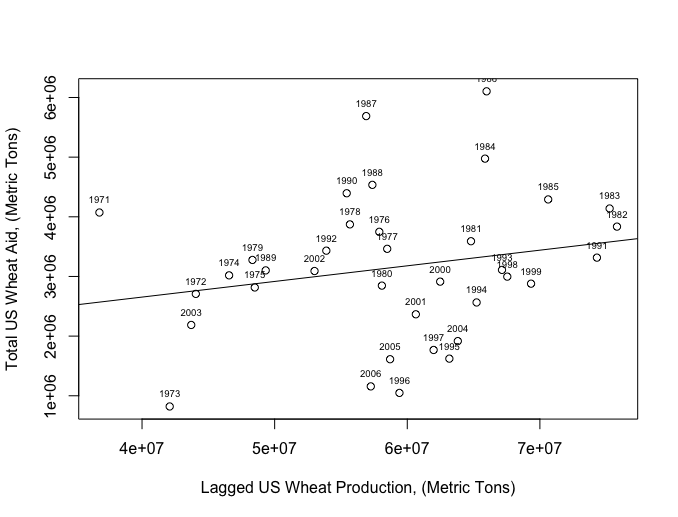
\includegraphics[scale=0.5]{wheatAidvsProd}
\label{wheataidprod}
\caption{Total US Wheat Aid vs Lagged US Wheat Production by year}
\end{figure}
 
The conclusion of the analysis in Nunn and Qian can be interpreted as US wheat production influences the incidence of conflict in countries in the subsequent year through food aid. Indeed, we can see this relationship directly in figure \ref{warwheatprod} the total frequency of conflict in all countries in our dataset against lagged US wheat production. 

\begin{figure}
\centering
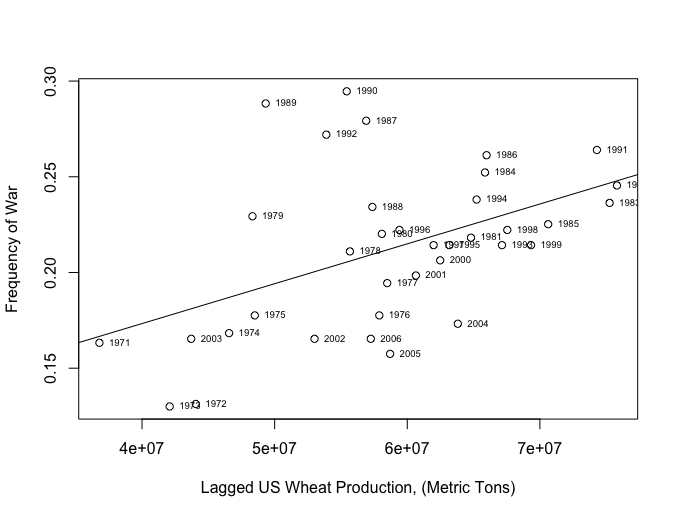
\includegraphics[scale=0.5]{warvsWheatProd}
\label{warwheatprod}
\caption{Frequency of War vs Lagged Wheat Production by Year}
\end{figure}

\section{Duplication of Regression Results}
We now proceed with our duplication of the main results of Nunn and Qian. 
\subsection{OLS}
We start by performing an OLS regression with model
\[C_{it} = \beta F_{it} \times \bar D_{i} + \x_{it} \gamma +  \delta_r t + \psi_{i} + \nu_{it}, \]
where $C_{it}$ is an indicator for the presence of conflict in country $i$ during year $t$, $F_{it}$ is the quantity of wheat aid shipped from the US to that country during that year, $\bar D_{i}$ is the average frequency of US provided aid to the country, $\x_{it}$ is a length $K$ vector of containing information about the country during that year, $\delta_r t$ denotes region specific time trends for the region $r$ the country is in (the region-year fixed effect), and $\psi_{i}$ denotes country specific effects. In total, as there are 125 countries in six regions in the dataset.\\

The we use five sets of $\x_{it}$, based on five sets of concerns raised by the authors:
\begin{enumerate}
\item[(1)] The baseline model where $\x_{it}$ is empty. The only controls in this model are fixed effects for countries and regions as well as regional trends. We will call this model 1. 
\item[(2)] There is concern about US wheat production and food aid being correlated with US economic cycles, US political cycles, and the oil price shocks during the 1970s, all three of which may influence the incidence of conflict in other countries. As a result, the authors add to model 1 indicators for each of these three variables, as well as their interaction with $\bar D_{i}$: US real per capita GDP, real oil prices, and an indicator that equals one in years that the US president is a Democrat. We will call this model 2. 
\item[(3)] The authors also raise concerns that weather conditions that impact US food aid are correlated with weather conditions in the recipient countries, which in turn may directly impact the incidence of conflict. As a result, they add in the average monthly temperature and monthly precipitation in the recipient country, as well as their interaction terms with $\bar D_{i}$, to control for these effects, totaling 48 additional terms. We add these terms to model 2 to obtain model 3. 
\item[(4)] The authors then raise concerns about the countries who are regular recipients of US food aid (that is, with higher values of $\bar D_{i}$) may differ from other countries in ways that relate to the risk of military conflict. In particular, the authors note that countries who receive more US food aid also tend to receive more of both US military aid and other economic aid from the US. These effects may not be adequately controlled for by the country-level fixed effects, as US military and economic aid may vary over time. As a result, the authors choose to also include  interaction of year fixed effects with (i) the average annual amount of per capita US military aid received by a country during the sample period and (ii) the average annual per capita amount of other forms of US economic aid (net of food aid). However, we were confused by this choice, both because none of the other terms involving the recipient country in the regression are per capita, and because it seems more sensible to include the amount of US military aid and US economic aid (net food aid) received by a country in the given year instead. As a result, we add the total amount of US military and US economic aid (net food aid) to model 3 to obtain model 4. 
\item[(5)] Finally, the authors note that US wheat production can affect international wheat prices, which may, in turn, affect conflict. As a result, the authors include the interaction of year fixed effects with a country’s (i) average per capita net imports of cereals over the sample period and (ii) average per capita production of cereals. We added these terms to model 4 to obtain model 5. 
\end{enumerate}
Finally, like the authors, we also consider the affects of food aid on only civil conflicts or interstate conflicts. We replace the dependent variable in model 5 with an indicator for civil conflicts and an indicator for interstate conflicts to obtain (6) model 6 and (7) model 7. 

The results for our OLS regressions are given in table \ref{ols}. Interestingly, some of the values we got were very slightly different from the authors', likely due to small differences in the regression setup and a slightly different choice of controls in models 4, 5, 6, and 7.  Notably, we find a very small but barely significant negative effect of wheat aid on all conflict, and an even smaller but much more significant negative effect of wheat aid on interstate conflict. 
\begin{table}
\centering
\scriptsize
\begin{tabular}{| l | c | c | c | c | c | c | c |}
\hline
& Model 1 & Model 2 & Model 3 & Model 4 & Model 5 & Model 6 & Model 7\\
\hline
Dependent Variable & All Conflict &  All Conflict &  All Conflict &  All Conflict & All Conflict & Intrastate & Interstate \\
\hline 
US Wheat Aid (1000 MT) & -0.00006 & -0.00007  & -0.00005  & -0.00008  & -0.00012  & 0.00002  & -0.00009 \\
~~p-value & (0.269) & (0.199) & (0.378) & (0.141) & (0.042) & (0.742) & (0.00092)\\
$R^2$ & 0.51 & 0.51 & 0.519 & 0.5203 & 0.535 & 0.509 & 0.365  \\
\hline
Controls:\\
~~Country FE & Yes & Yes & Yes & Yes & Yes & Yes & Yes \\
~~Region-year FE & Yes & Yes & Yes & Yes & Yes & Yes & Yes \\
~~US GDP per capita$\times \bar D_{it}$  & No & Yes & Yes & Yes & Yes & Yes & Yes \\
~~Dem. President $\times \bar D_{it}$ & No & Yes & Yes & Yes & Yes & Yes & Yes \\
~~Oil Price $\times \bar D_{it}$ & No & Yes & Yes & Yes & Yes & Yes & Yes \\
~~Temp. and Percipitation & No & No & Yes & Yes & Yes & Yes & Yes \\
~~Temp. and Percip. $\times \bar D_{it}$& No & No & Yes & Yes & Yes & Yes & Yes \\
~~Total US military aid  & No & No & No & Yes & Yes & Yes & Yes \\
~~Total US econ. aid & No & No & No & Yes & Yes & Yes & Yes \\
~~Avg. cereal imports $\times$ year FE & No & No & No & No & Yes & Yes & Yes \\
~~Avg. cereal prod. $\times$ year FE & No & No & No & No & Yes & Yes & Yes \\
\hline
\end{tabular}
\label{ols}
\normalsize
\caption{OLS estimates of the 
effect of food aid on conflict under different models. p-values are provided in parentheses.}
\end{table}
\subsection{2SLS }
In addition to the model above, we also perform a 2SLS regression with US wheat production during the previous year as an instrument for food aid. The model used is:
\begin{align*}
F_{it} &= \alpha P_{t-1}\times \bar D_{i} +  \x_{it} \gamma +  \delta_r t + \psi_{i} + \epsilon_{it}\\
C_{it} &= \beta  F_{it} \times \bar D_{i}+ \x_{it} \gamma +  \delta_r t + \psi_{i} + \nu_{it}
\end{align*}
Where $P_{t-1}\times \bar D_{i}$ is the US production of wheat in the preceding year, times the frequency the country receives food aid from the US. We use the same five sets of $\x_{it}$ as in the 2SLS. In addition, we will also consider the effects on intrastate and interstate conflicts, using the final, most inclusive set of controls. As before, we will label our models 1 through 7. \\

We report the results of the first and second stage regressions in table \ref{2sls}. As with our OLS estimates, our 2SLS estimated parameters are also slightly different from Nunn and Qian's, likely due to small differences in the regression setup and the choice of controls for models 4 through 7. As with their analysis, our analysis finds significant positive effects of wheat aid on the incidence of all armed conflict and on intrastate conflict. However, we also find a significant but smaller effect negative effect of US wheat aid on international conflict. 

\begin{table}
\centering
\scriptsize
\begin{tabular}{| l | c | c | c | c | c | c | c |}
\hline
& Model 1 & Model 2 & Model 3 & Model 4 & Model 5 & Model 6 & Model 7\\
\hline
Dependent Variable (first stage) & \multicolumn{7}{|c|}{US Wheat Aid (1000 MT)}\\
\hline 
Lagged US Wheat Prod (1000 MT) & 0.0026 & 0.0033  & 0.0034  & 0.0033  & 0.0035  & 0.0035  & 0.0035  \\
~~~~$\times \bar D_{i}$ & & & & & & & \\
~~p-value & (0.000003) & (0.000009) & ($2.54 \cdot 10^{-10}$) & ($2.43 \cdot 10^{-10}$) & ($2.06 \cdot 10^{-10}$) & ($2.06 \cdot 10^{-10}$) & ($2.06 \cdot 10^{-10}$)\\
$R^2$ & 0.511 & 0.519 & 0.527 & 0.553 & 0.559 & 0.559 & 0.559 \\
\hline
Dependent Variable (second stage) & All Conflict &  All Conflict &  All Conflict &  All Conflict & All Conflict & Intrastate & Interstate \\
\hline 
Fitted US Wheat Aid (1000 MT) & 0.00271 & 0.00279  & 0.00231 &0.00155 & 0.00110  & 0.00152  & -0.00059 \\
~~p-value & (0.000001) & ($3.6 \cdot 10^{-7}$) & (0.000016) & (0.00103) & (0.03512) & (0.000526) & (0.00513)\\
$R^2$ & 0.516 & 0.517 & 0.525 & 0.525 & 0.530 & 0.513 & 0.365  \\
\hline
Controls:&  \multicolumn{7}{|c|}{~}\\
~~Country FE & Yes & Yes & Yes & Yes & Yes & Yes & Yes \\
~~Region-year FE & Yes & Yes & Yes & Yes & Yes & Yes & Yes \\
~~US GDP per capita$\times \bar D_{it}$  & No & Yes & Yes & Yes & Yes & Yes & Yes \\
~~Dem. President $\times \bar D_{it}$ & No & Yes & Yes & Yes & Yes & Yes & Yes \\
~~Oil Price $\times \bar D_{it}$ & No & Yes & Yes & Yes & Yes & Yes & Yes \\
~~Temp. and Percipitation & No & No & Yes & Yes & Yes & Yes & Yes \\
~~Temp. and Percip. $\times \bar D_{it}$& No & No & Yes & Yes & Yes & Yes & Yes \\
~~Total US military aid  & No & No & No & Yes & Yes & Yes & Yes \\
~~Total US econ. aid & No & No & No & Yes & Yes & Yes & Yes \\
~~Avg. cereal imports $\times$ year FE & No & No & No & No & Yes & Yes & Yes \\
~~Avg. cereal prod. $\times$ year FE & No & No & No & No & Yes & Yes & Yes \\
\hline
\end{tabular}
\label{2sls}
\normalsize
\caption{First stage estimates of the effect of lagged production on US wheat aid, as well as second stage estimates of the effect of food aid on conflict under different models. p-values are provided in parentheses.}
\end{table}


\section{Testing for Heteroscedasticity}
All of the p-values and standard errors reported in the paper, as well as those reported above, assume homoscedascedasticity. Here, we check if the dataset contains evidence of heteroscedasiticty by examining the models with all the explanatory and control variables - namely, models 5 through 7. Indeed, from now on, we will only focus on the effects of models 5 through 7, from which they draw the bulk of their significant results. \\

We start with graphically examining the residuals from the OLS regressions with models 5 through 7 in figures 3, 4, and 5. There is some evidence of heteroscedasiticity in models 5 and 6, and much clearer evidence for  heteroscedasiticity in model 7, however. \\
 
 \begin{figure}
\centering
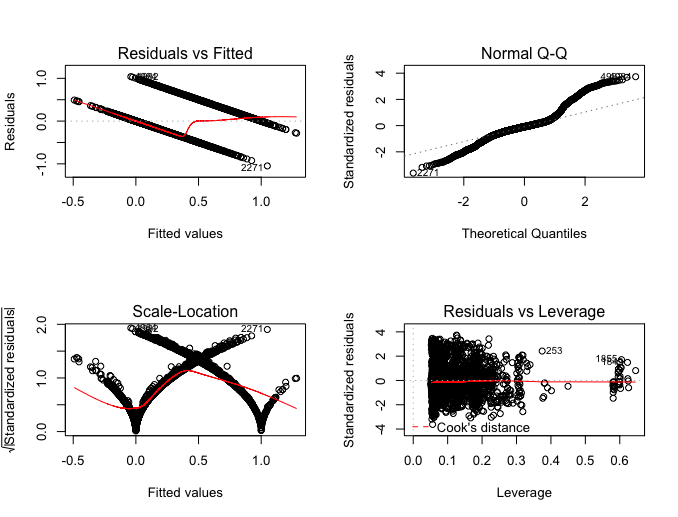
\includegraphics[scale=0.5]{model5Resid}
\label{model5resid}
\caption{Residual plots for OLS with model 5. There exists some evidence of heteroscedasicity from the Scale-Location and Residuals vs Fitted plots.}
\end{figure}

 \begin{figure}
\centering
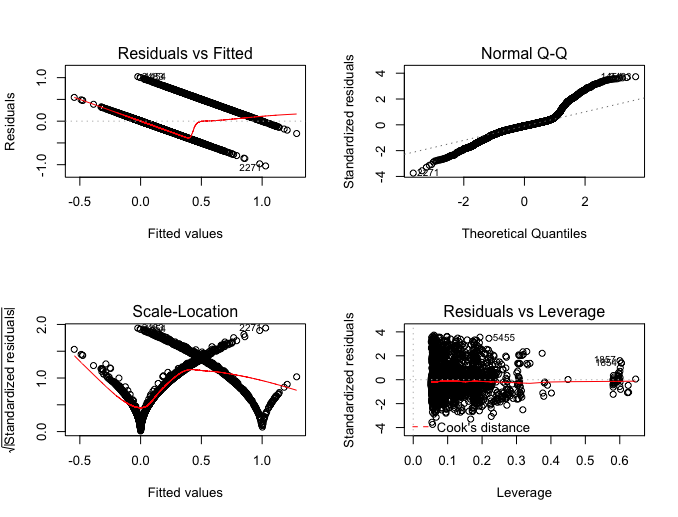
\includegraphics[scale=0.5]{model6Resid}
\label{model6resid}
\caption{Residual plots for OLS with model 6. As with the residuals for model 5, there exists some evidence of heteroscedasicity from the Scale-Location and Residuals vs Fitted plots.}
\end{figure}

 \begin{figure}
\centering
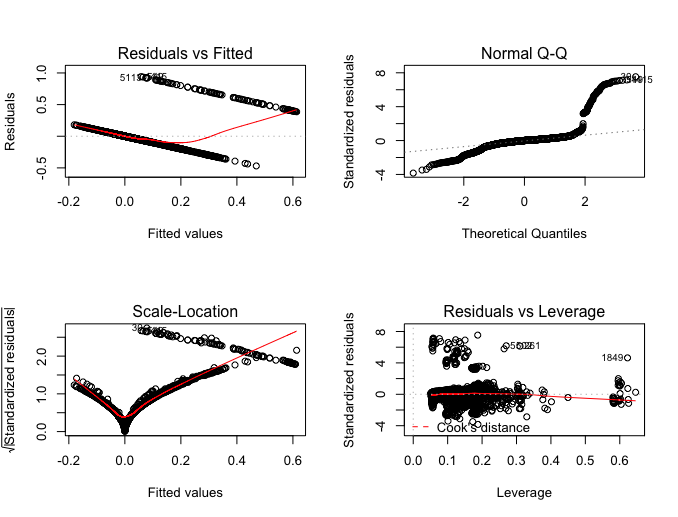
\includegraphics[scale=0.5]{model7Resid}

\caption{Residual plots for OLS with model 7. There is now clear evidence of heteroscedasiticty from both the Normal Q-Q plot and the Scale-Location plot.}
\label{model7resid}
\end{figure}

In order to statistically test for heteroscedasticity, we use the Breusch-Pagan test covered in class. We regress the squared OLS residuals of each of the models against the explanatory variables, then use the fact that the Lagrange multiplier test statistic has a chi-square distribution with 470 degrees of freedom under the null hypothesis of homoscedasticity. We report our results in table \ref{Breusch}.\\

\begin{table}
\center 
\begin{tabular}{| l | c | c | c|}
\hline
~ & Model 5 & Model 6 & Model 7 \\
\hline 

F-statistic & 2.931 & 3.571 & 3.289 \\
~~p-value & $ < 2.2\cdot10^{-16}$ & $< 2.2\cdot10^{-16}$ 
&$< 2.2\cdot10^{-16}$\\
$R^2$ &  0.27 & 0.311 &  0.293 \\
$n$ &  4089 & 4089 & 4089 \\
$nR^2$ & 1103.97 & 1270.0 & 1119.183 \\
~~p-value & 0 & 0 & 0\\
\hline
\end{tabular}
\label{Breusch}
\caption{Results of regressing squared OLS residuals against the explanatory variables in each of the three models. All three possess significant evidence of heteroscedasticity, whether from the extremely low p-value on the F-statistic for the regression, or for the extremely high value (and low p-value) for the Breusch-Pagan test statistic $nR^2$.}
\end{table}

As a follow up, we perform the same test using the 2SLS residuals of each of the models against the explanatory variables. As before, we use the fact that the test statistic is Chi-square distributed with 470 degrees of freedom under the null hypothesis. We report our results in table \ref{Breusch2s}.\\

\begin{table}
\center 
\begin{tabular}{| l | c | c | c|}
\hline
~ & Model 5 & Model 6 & Model 7 \\
\hline 

F-statistic & 2.815 & 3.448 & 3.308 \\
~~p-value & $ < 2.2\cdot10^{-16}$ & $< 2.2\cdot10^{-16}$ 
&$< 2.2\cdot10^{-16}$\\
$R^2$ &  0.2828 & 0.3036 &  0.295 \\
$n$ &  4089 & 4089 & 4089 \\
$nR^2$ & 1156.37 & 1241.62 & 1206.51 \\
~~p-value & 0 & 0 & 0\\
\hline
\end{tabular}
\label{Breusch2s}
\caption{Results of regressing squared 2SLS residuals against the explanatory variables in each of the three models. All three possess significant evidence of heteroscedasticity, whether from the extremely low p-value on the F-statistic for the regression, or for the extremely high value (and low p-value) for the Breusch-Pagan test statistic $nR^2$.}
\end{table}

From the results of both the graphical examination and the test, we can conclude that the dataset exhibits strong signs of heteroscedasticity. This strongly implies that standard-error and p-value calculations for both the OLS and 2SLS estimates may not be accurate, and so they should be redone with heteroscedasiticty-robust estimators.\\

We do exactly that, reporting the heteroscedasiticity-robust estimates of parameters from models 5 through 7 for both OLS and 2SLS in table \ref{HCstuff}. Note that the robust standard errors are about 10\% larger than the normal standard errors, and  substituting an robust p-value calculation for the original p-value calculation leads to the effect of US Wheat Aid in model 5 no longer being significant for either OLS or 2SLS. However, the effect for model 6 is still extremely significant, meaning that the authors' main conclusion - that "US wheat aid increases the chance of civil conflict" - still holds. Nonethelss, this suggests that their results may not be as robust as they claim it to be.  

\begin{table}
\center 
\begin{tabular}{| l | c | c | c|}
\hline
~ & Model 5 & Model 6 & Model 7 \\
\hline 

OLS Estimate of US Wheat Aid Effect (Per 1000 MT) & -0.00012  & 0.00002 & -0.00009 \\
~~Standard Error & 0.000060 & 0.000057 & 0.000027 \\
~~Standard Error (HC0) & 0.000068 & 0.000068 & 0.000036 \\
~~Standard Error (HC1) & 0.000072 & 0.000072 & 0.000038\\
~~Standard Error (HC2) & 0.000073 & 0.000073 & 0.000039 \\
~~p-value & $ 0.042 $ & $0.742$ 
&$0.000092$\\
~~p-value (HC1 standard errors)& $ 0.092$ & $0.794$ 
&$0.0198$\\
\hline 
2SLS Estimate of US Wheat Aid Effect (Per 1000 MT) & 0.00110 & 0.000152 & 3.308 \\
~~Standard Error & 0.000543 & 0.000437 & 0.000210\\
~~Standard Error (HC0) & 0.000567 & 0.000470 & 0.000241\\
~~Standard Error (HC1) & 0.000603 & 0.000499 & 0.000255\\
~~Standard Error (HC2) & 0.000621 & 0.000512 & 0.000265 \\
~~p-value & $ 0.035 $ & $0.0053$ 
&$0.0051$\\
~~p-value (HC1 standard errors)& $ 0.092$ & $0.0024 $ 
&$0.0198$\\
\hline
\end{tabular}
\label{HCstuff}
\caption{Comparision of original standard errors and p-values to heteroscedasticity-robust standard errors and p-values. Notice that the 2SLS estimates for model 5 are no longer significant. }
\end{table}

\section{Testing for Endogeneity}
Finally, we consider the question of whether the author's use of two-stage least squares is appropriate. Namely, is there evidence for endogeneity in our OLS procedure? (Notice that the instrument is already significantly marginally correlated with supposedly endogenous variable from our previous results.) \\

\begin{table}
\center 
\begin{tabular}{| l | c | c | c|}
\hline
~ & Model 5 & Model 6 & Model 7 \\
\hline 

$F_{Haussmann}$ & 23.096 & 19.161 & 1.225 \\
~~p-value & $0.0000015$ & $0.0000120$ 
&$0.2684$\\
\hline
\end{tabular}
\label{Haussman}
\caption{The (homoscedastic) test statistic from the Hausman test for endogeneity, and its p-value. There exists significant evidence for endogeneity in for both the intrastate and all conflict variable, but not for the intrastate model. }
\end{table}

\begin{table}
\center 
\begin{tabular}{| l | c | c | c|}
\hline
~ & Model 5 & Model 6 & Model 7 \\
\hline 

$F_{Haussmann}$ & 32.0165 & 19.058 & 1.930 \\
~~p-value & $0.0000016$ & $0.000013$
&$0.1647$\\
\hline
\end{tabular}
\label{HaussmanHC}
\caption{The (heteroscedasticity-robust, using HC1) test statistic from the Hausman test for endogeneity, and its p-value. Note that the results are very similar  exists significant evidence for endogeneity in for both the intrastate and all conflict variable, but not for the intrastate model. }
\end{table}

We begin by performing the Hausman test for endogeneity. We regress the target variables of each of the models against the OLS explanatory variables, plus the residuals of the first stage regressions from 2SLS, and then compare the test statistic to the Chi-square distribution with 1 degree of freedom (as there is a single variable and one instrument). The results are presented in table \ref{Haussmann}. We find that there does seem to exist endogeniety for the all conflict variable and intrastate variable, which helps justify the author's use of 2SLS for at least models 5 and 6. \\

Since we previously uncovered evidence of heteroscedasticity, we also repeat this test with the heteroscedasiticity-robust standard error estimator HC1 from the sandwich package, though we find it makes little difference to the results of the test. \\



\section{Conclusion and Future work}
In this work, we attempted to duplicate part of the analysis of Nunn and Qian's 2014 paper on the effect of US Food Aid on Civil Conflict. After duplicating (to a large part) their analysis, we found that their dataset exhibited significant signs of heteroscedasticity, prompting us to switch to heteroscedasiticity-robust standard errors. We found that one of their main results - that there was a significant effect of US food aid on the total incidence of large-scale armed conflict - disappeared following this switch, but their overall conclusion of "US wheat aid increasing the chance of civil conflict" still held. Nonetheless, we believe this raises some question as to the robustness of their result. \\

One particularly interesting research avenue that follows from Nunn and Qian's work is to use a different model to explore the effects. Instead of using a linear regression, it may make more sense to use a logistic regression to estimate the effects of food aid on war. Nunn and Qian begin on this path by building a logistic discrete time hazard model to model the effect of aid on the duration of armed conflict, but we believe that the main analysis could also benefit from being put into a logistic regression framework. 

\end{document}
